\documentclass[class=article , crop=false, titlepage, twoside, multi={itemize, figure, verbatim}, float=false]{standalone}
\usepackage{caption}
\usepackage{import} % Required for importing other .tex docs.  (import uses everything bw Begin and End Doc)
\usepackage{float} % Required for specifying the exact location of a figure or table
\usepackage{graphicx} % Required for including images
\usepackage{wrapfig}
\usepackage[pdftex,breaklinks,colorlinks=true,linkcolor=black,citecolor=blue,urlcolor=red,linktocpage=false,pagebackref=true,filecolor=magenta]{hyperref}%http://www.tug.org/applications/hyperref/manual.html#x1-100003.6
\usepackage{cite}
\usepackage[toc,title,page]{appendix}
\usepackage{pdfpages} % enables loading a pdf into the doc
\usepackage{makeidx}
\usepackage{glossaries} % must be after hyperref
\usepackage{blindtext}
\usepackage{enumitem}
%\usepackage{caption}

%\setlist[description]{leftmargin=\parindent,labelindent=\parindent}

%\renewcommand*{\bibname}{References} % renames the bibliography

\newcommand{\HRule}{\rule{\linewidth}{0.5mm}} % Command to make the lines in the title page

\graphicspath{{img/}{GIS_ChampionSection/img/}{awardsChapter/GIS_ChampionSection/img/}{brandPart/awardsChapter/GIS_ChampionSection/img/}{img/}{pairedProgSection/img/}{methodChapter/pairedProgSection/img/}{methodPart/methodChapter/pairedProgSection/img/}{documentationSection/img/}{methodChapter/documentationSection/img/}{methodPart/methodChapter/documentationSection/img/}{docStorageOrgSection/img/}{methodChapter/docStorageOrgSection/img/}{methodPart/methodChapter/docStorageOrgSection/img/}{QGisSection/img/}{toolsChapter/QGisSection/img/}{servicePart/toolsChapter/QGisSection/img/}{ESRISection/img/}{toolChapter/ESRISection/img/}{servicePart/toolChapter/ESRISection/img/}{../../../../source/}{../../source/}{servicePart/applicationsChapter/treasurerSection/img/}}

%\setlength\parindent{0pt} % eliminates indents


\def\titlename{Forfeiture Data Collection\\ \medskip\large Mobile App with Collector for ArcGIS}

\title{\HRule % Horizontal Line added
\\[.4cm] % space
\begin{figure}[H] % included image
\begin{center}	% centered horizontally
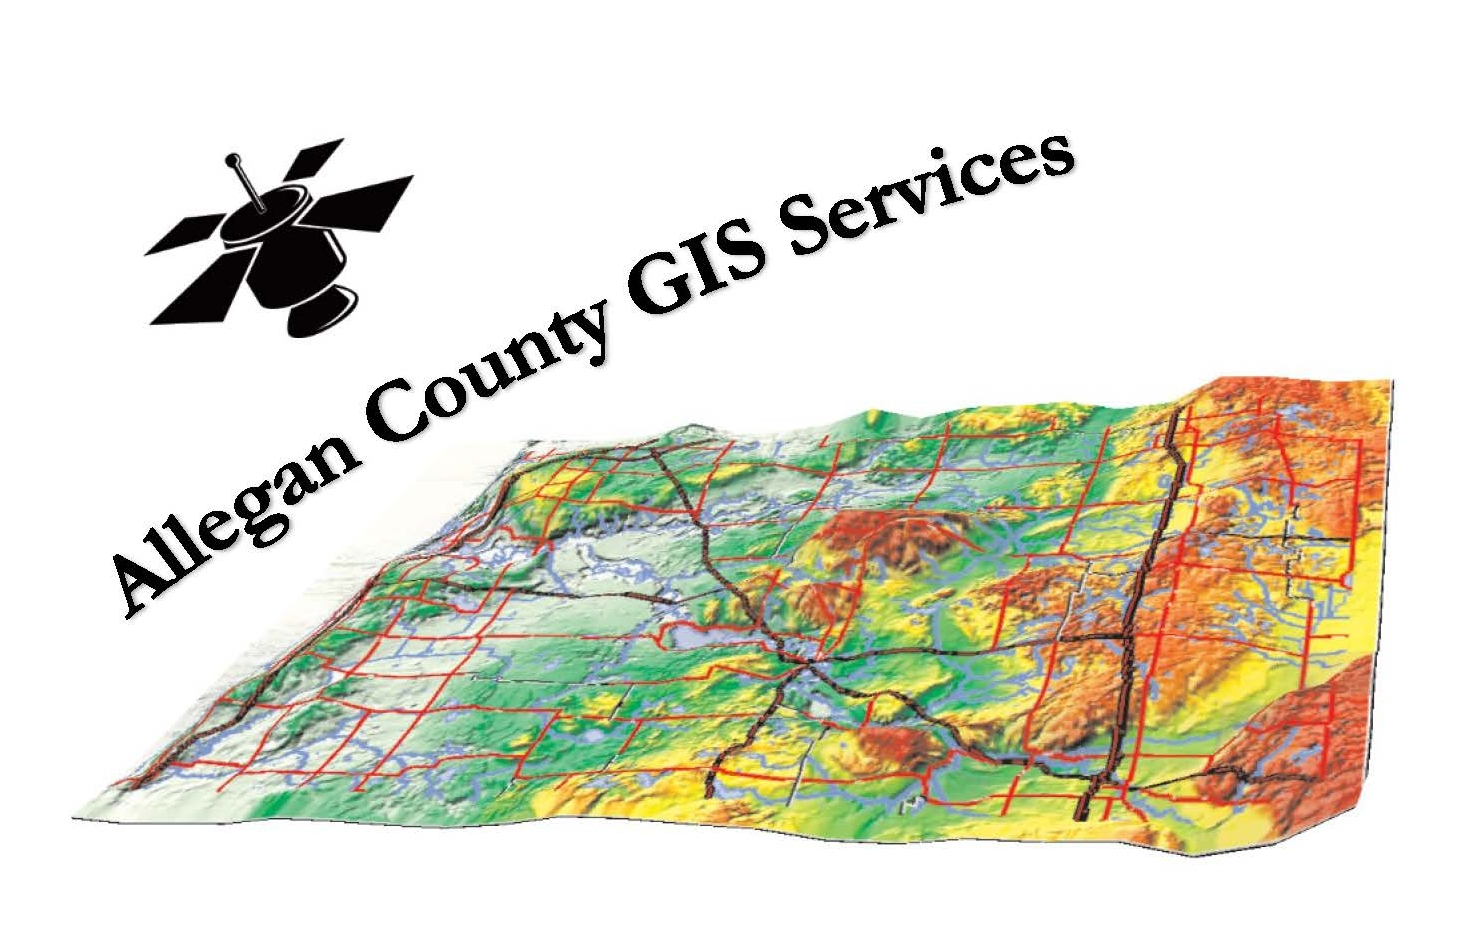
\includegraphics[scale=.45]{GIS_Logo_better.jpg}
\end{center}
\end{figure}
\Huge \bfseries \titlename \\ % Title text
\HRule \\[.4cm] % Horizontal Line added
\author{\Large Allegan County GIS \\\Large www.allegancounty.org/gis} % defines author
}  % inputs common title
\setcounter{tocdepth}{5}  % subparagraph and down
\begin{document}% document begins

\ifstandalone
\maketitle % creates title page
\clearpage
\tableofcontents % creates TOC
\clearpage
\fi

\subsection{Forfeiture Data Collection}

\subsubsection{Problem and Analysis}

\paragraph{Background}
Treasurer department has an annual responsibility to properly document the tax forfeiture process.  The LIS Department built an application in MS Access and MapInfo that consumed a daily export from BSA and was deployed to the field on a laptop.  A digital camera was used for site photos and later imported into the laptop.

\paragraph{Statement of Problem}
Current Tax Forfeiture workflow is built on MapInfo software which has been replaced by ESRI software.  The Forfeiture data collection application must be recreated in the ESRI framework.


\paragraph{Analysis}
Tax Forfeiture Application will facilitate:

\begin{itemize} %1

\item Mobile data collection on handheld device via Collector for ArcGIS configured with Allegan County GIS Portal  (\textbf{device app})

\begin{itemize} %2

\item Device app will:

\begin{itemize} %3

\item Synchronize with data in the office (online)
\item Navigate to forfeiture sites (offline)
\item Collect data and photos of forfeiture sites (offline)
\item Synchronize the collected data with data in the office (online)
\end{itemize} %3

\end{itemize} %2

\item Daily form production and printing for each site visited with required data and images.

\end{itemize} %1

\clearpage
\subsubsection{Design}

\paragraph{Overview}The Forfeiture Data Collection Application uses BSA, ArcGIS Desktop, ArcGIS Collector for Android, and ArcGIS Portal web maps and apps to enable forfeiture data collection.  A daily routine is supported that maintains forfeiture parcel data through the notification period.
\begin{center}
    %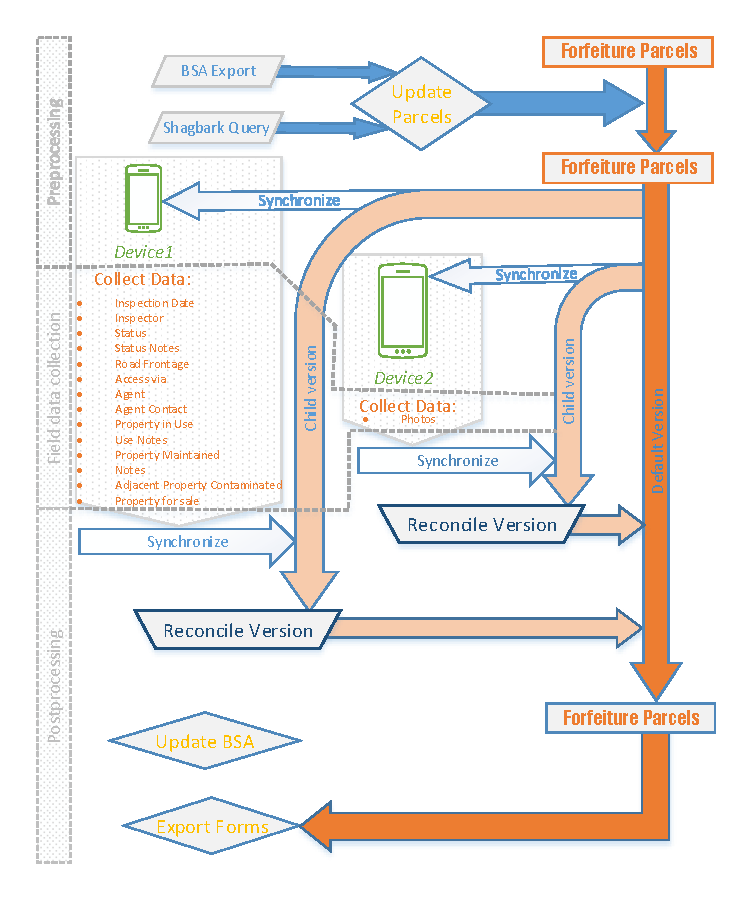
\includegraphics[width=1\textwidth]{DesignFlowChart}
    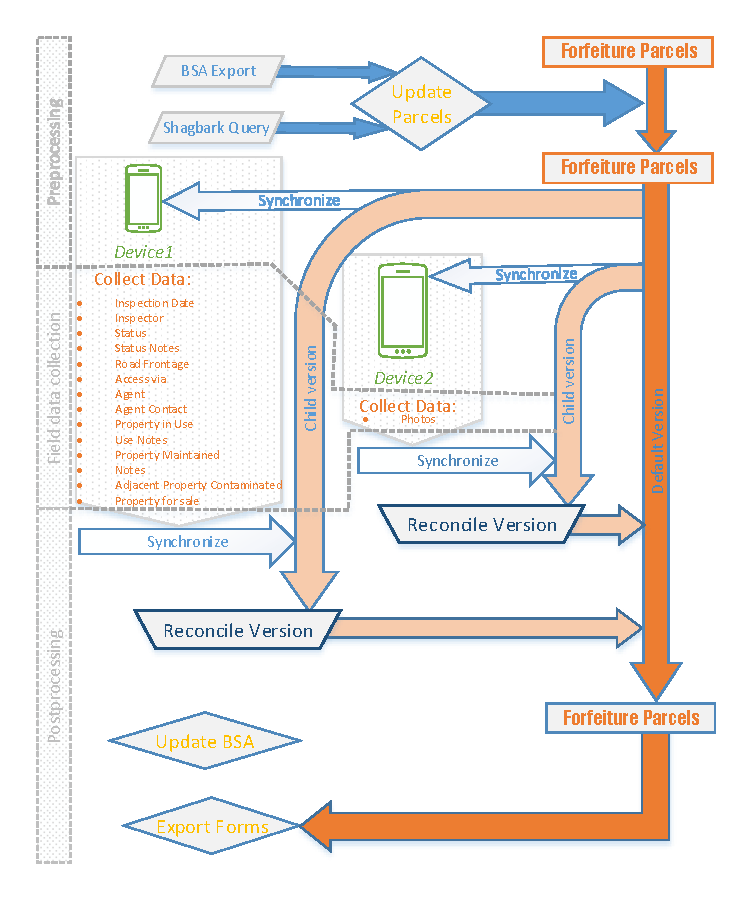
\includegraphics{DesignFlowChart}
    \captionof{figure}{Project Design}
    
\end{center}


\subparagraph{BSA data export}Details of parcels in the forfeiture process are managed in BSA Delinquent Tax.net.  The Treasurer office has a BSA export the parcels that need a site visit.  Export of the updated list is the beginning of the daily routine in this workflow.

\subparagraph{ArcGIS Desktop tasks}Tools are designed to preprocess and postprocess forfeiture parcel data for fieldwork.  The user will execute a preprocess script tool that prepares the data for field deployment.  After fieldwork, a post process script tool syncronizes data from the fieldwork with the live data on the Allegan County network. 

\subparagraph{ArcGIS Collector}A free mobile application developed and tested on Android is deployed to the field for data collection.  The application is configured to work offline(without an internet or cellular connection) by syncronizing before and after fieldwork.

\subparagraph{ArcGIS Portal Webmaps and Apps}Live data from a publishing (replica of ACPro) enterprise geodatabase (ACPub) running on SQL Server database server (acintsql01) is provided through a feature service (REST service)  named TaxReversionParcels.  A webmap called Forfeiture Field Map consumes the TaxReversionParcels feature service exposing the forfeiture parcels, for editing.  The Forfeiture Field Map is configured to work in the ArcGIS Collector App.  The app downloads the webmap, allowing the user to collect the necessary information on each forfeiture parcel in the field disconnected and uploads the changes when reconnected. 

\paragraph{Forfeiture Data Collection}

Three parts of the daily routine:
\begin{enumerate}
\item Pre-processing (in the office):

\begin{itemize}
\item Export current forfeiture list from BSA
\item Update webmap layers with results from BSA export
\item Synchronize from webmap layers to field collection device \textbf{(device app)}
\end{itemize}

\item Field data collection with device app:

\begin{itemize}
\item Support navigation to forfeiture sites
\item Provide a checklist of data points about the site
\item Attach photos to the site
\item Save results for synchronization in post-processing
\end{itemize}

\item Post-processing (in the office)

\begin{itemize}
\item Synchronize data and images collected in device app to webmap layers

\end{itemize}
\end{enumerate}

\paragraph{Backend data details}
\subparagraph{Location of production data}

\begin{center}
    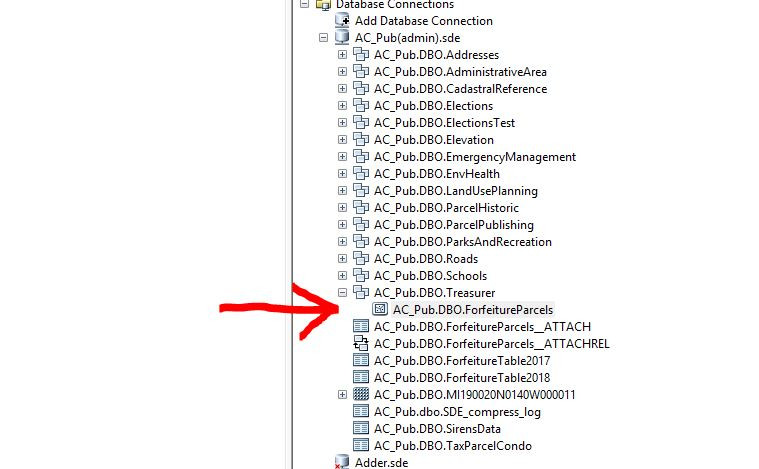
\includegraphics[width=1\textwidth]{ForfParcelsCatalog2}
    \captionof{figure}{live data}
    \label{img:g}
\end{center}

\subparagraph{ForfeitureParcels feature class}



\paragraph{Collector Setup Details}

\subparagraph{Install Collector for ArcGIS} Available from the Google Play Store

\subparagraph{App setup}

\begin{itemize}
\item Connect to Allegan County GIS

\begin{itemize}
\item Sign In : enter this website address

\begin{verbatim}
https://gis.allegancounty.org/portal_webadaptor
\end{verbatim}

\item Username is JMorris or CAndress
\item Password: (enter password)

\centering 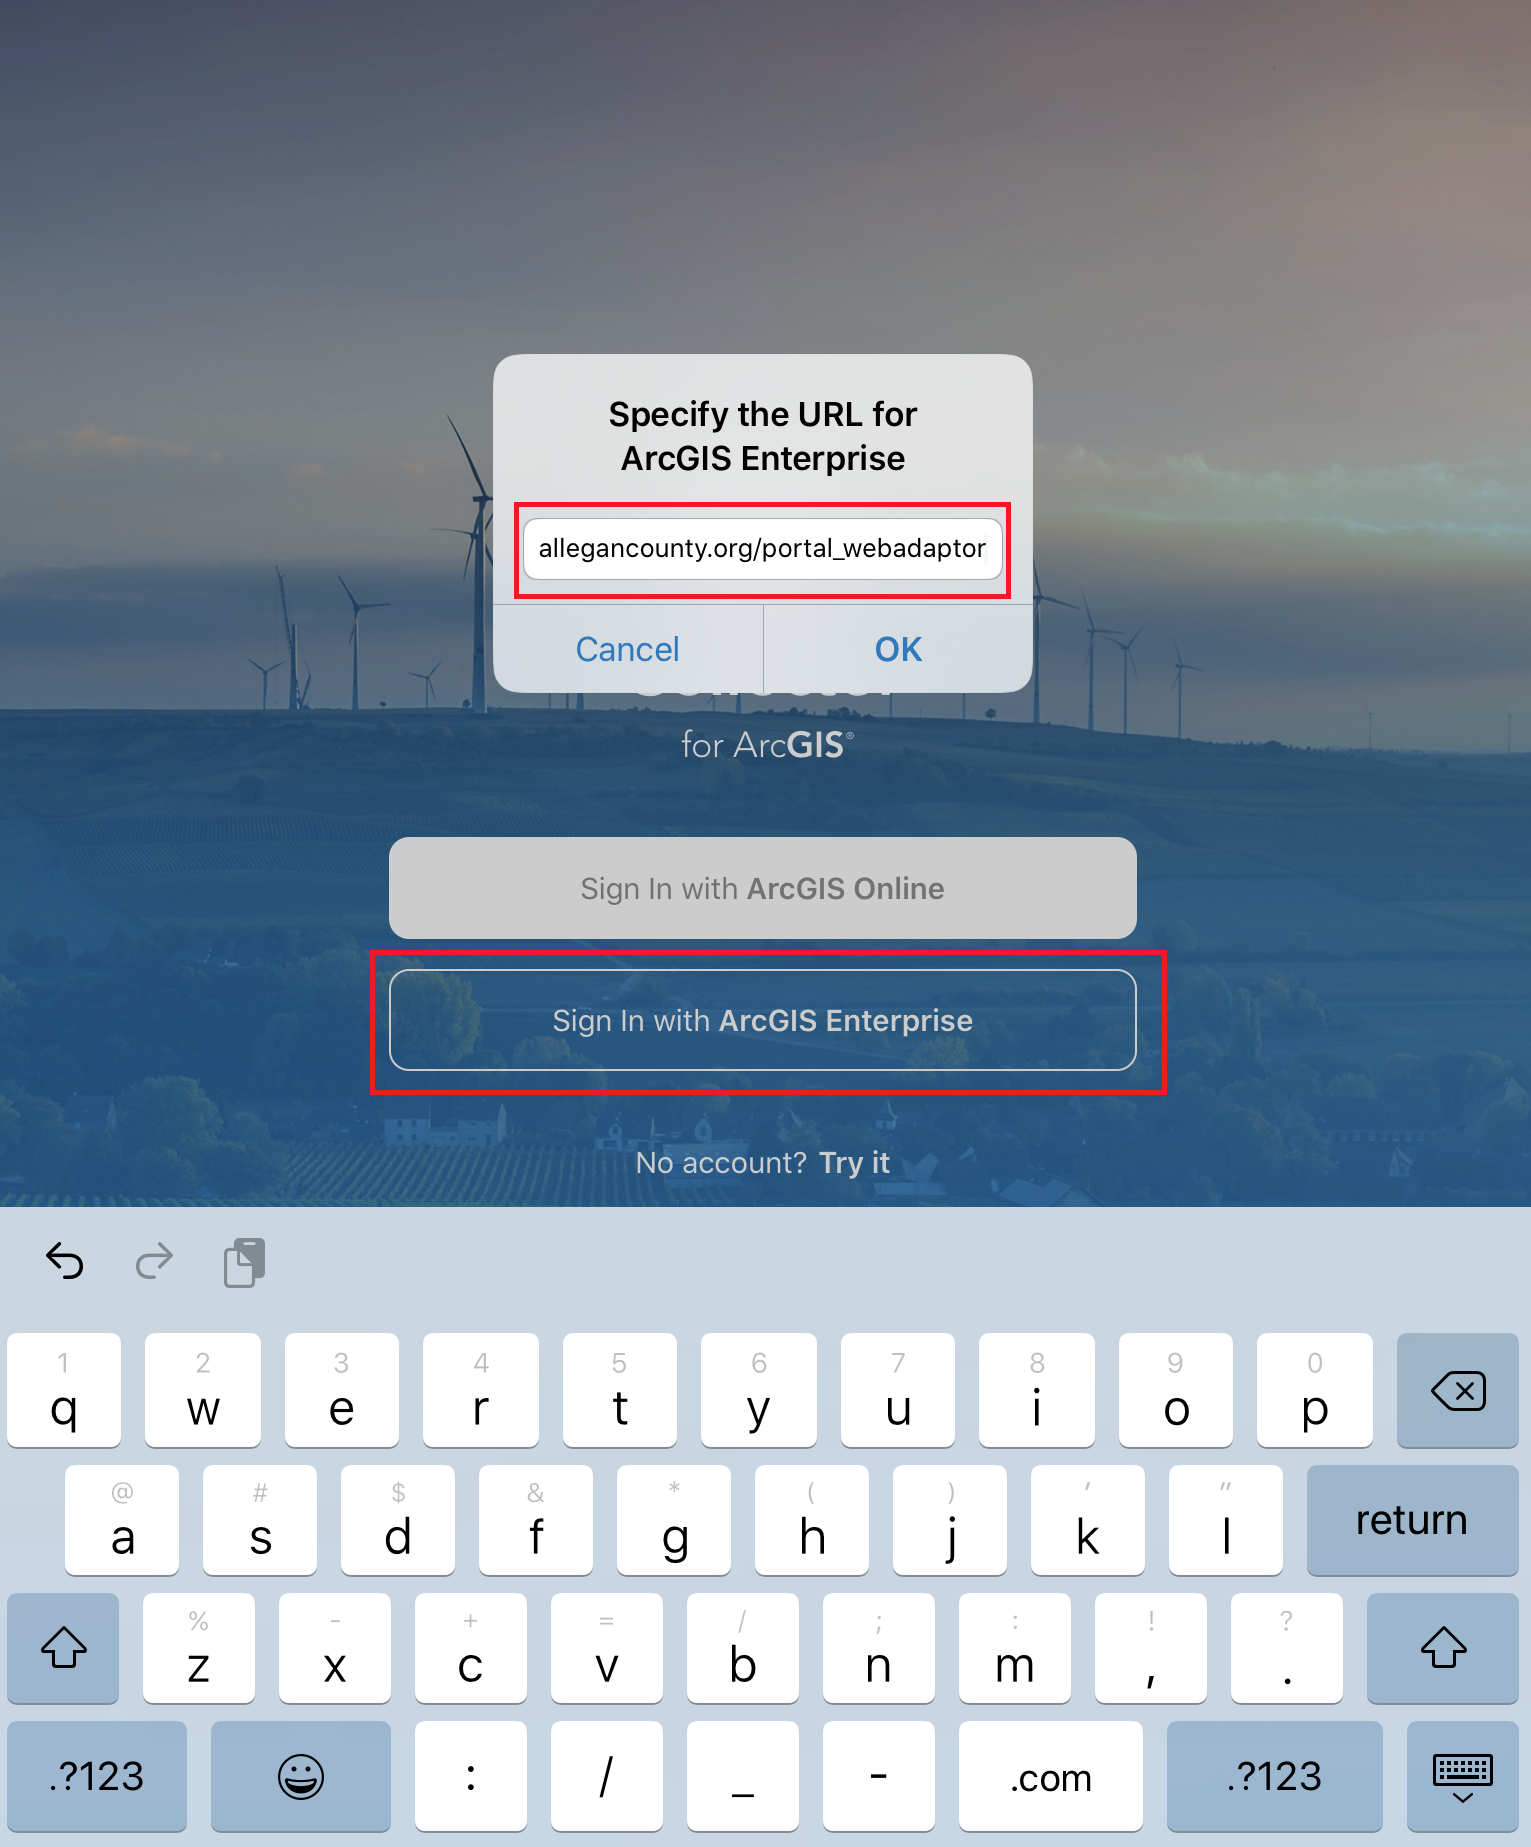
\includegraphics[width=4in]{CollectorConnection}
\captionof{figure}{Collector Connection}
%label{img:g}
\end{itemize}

\item Find the map Forfeiture Field Map under Treasury Services
\item Download the field map
\item Select area needed and detail needed


\end{itemize}

\subparagraph{Synchronize app}

\paragraph{Webmap details}

\clearpage
\subsubsection{Hard Copy Record}
\clearpage
\subsubsection{User Manual}
\paragraph{Preprocessing}

\paragraph{fieldwork}

\paragraph{postprocessing}

\subparagraph{Sync Edits}

\subparagraph{reconcile Versions}

\subparagraph{print forms for sites visited}

\subparagraph{update BSA}

\clearpage
\subsubsection{Software}
\clearpage
\end{document}